\documentclass[conference]{IEEEtran}
% ---------------------------------------------------------------------------
% RiskShare: Risk-Adaptive Threshold Secret Sharing with Fresh Cryptographic
% Epochs over Traceable Asmuth--Bloom Shares
% Build:  tectonic main.tex     (or: pdflatex, bibtex, pdflatex x2)
% ---------------------------------------------------------------------------
\usepackage[T1]{fontenc}
\usepackage{amsmath,amssymb,amsfonts,amsthm}
\usepackage{graphicx}
\usepackage[caption=false,font=footnotesize]{subfig}
\usepackage{booktabs,multirow}
\usepackage{algorithm}
\usepackage{algpseudocode}
\usepackage{xcolor}
\usepackage{tikz}
\usetikzlibrary{arrows.meta,positioning,shapes.geometric,fit,backgrounds,calc,shadows}
\usepackage{pgfplots}
\pgfplotsset{compat=1.18}
\usepgfplotslibrary{groupplots}
\usepackage{url}
\usepackage[hidelinks]{hyperref}
\usepackage{cite}

% ----- colours -------------------------------------------------------------
\definecolor{rsblue}{HTML}{2B6CB0}
\definecolor{rsteal}{HTML}{2C9AA8}
\definecolor{rsorange}{HTML}{DD6B20}
\definecolor{rsred}{HTML}{C53030}
\definecolor{rsgreen}{HTML}{2F855A}
\definecolor{rsgray}{HTML}{4A5568}
\definecolor{rslight}{HTML}{EDF2F7}

\pgfplotsset{
  rsaxis/.style={
    tick label style={font=\scriptsize},
    label style={font=\footnotesize},
    legend style={font=\scriptsize, draw=none, fill=none},
    grid=major, grid style={gray!20},
    axis line style={gray!60},
  },
}

\newtheorem{definition}{Definition}
\newtheorem{proposition}{Proposition}
\newcommand{\Z}{\mathbb{Z}}
\newcommand{\RS}{\textsc{RiskShare}}
\newcommand{\DEK}{\mathsf{DEK}}
\newcommand{\Enc}{\mathsf{Enc}}
\newcommand{\Dec}{\mathsf{Dec}}

\begin{document}

\title{RiskShare: Risk-Adaptive Threshold Secret Sharing\\ via Fresh Cryptographic Epochs over\\ Traceable Asmuth--Bloom Shares}

\author{
\IEEEauthorblockN{Akshai Praveen}
\IEEEauthorblockA{Roll No.\ 231210009\\
\textit{Department of Computer Science and Engineering}\\
\textit{National Institute of Technology Delhi}\\
New Delhi, India}
\and
\IEEEauthorblockN{Ayush Karn}
\IEEEauthorblockA{Roll No.\ 231210032\\
\textit{Department of Computer Science and Engineering}\\
\textit{National Institute of Technology Delhi}\\
New Delhi, India}
}

\maketitle

% ===========================================================================
\begin{abstract}
Threshold secret sharing protects a key by splitting it among $n$ servers so that any $t$ of them can recover it, but the threshold $t$ is fixed when the shares are created. Operational risk, by contrast, changes over time: authentication failures, invalid shares and missed heartbeats indicate that some servers may be compromised. We present \RS{}, an applied extension that couples an explainable, time-decayed risk score to the reconstruction threshold of the traceable Asmuth--Bloom schemes of Leslie and Dutta (ABSS-I/II, TTSS-I/II). Because an existing share set cannot be ``relabelled'' to a stricter threshold, \RS{} treats every threshold change as a \emph{fresh cryptographic epoch}: a new data-encryption key, AES-256-GCM re-encryption bound to the epoch, a new share generation at the target threshold, all-node distribution acknowledgement and atomic activation, with fail-closed behaviour on error. We implement the full stack---CRT-based sharing, elliptic-curve-committed tracing on P-384/P-521, a five-node share plane with HMAC-authenticated, replay-protected requests and signed responses, a hash-chained audit log, a FastAPI control plane and a web Control Room. In 500 scripted scenarios over five independent key generations, the adaptive policy matched the scripted attacker-reconstruction rate of a fixed 4-of-5 threshold (20\%) while raising legitimate recovery from 40\% to 48\%; reconstruction took about 4.1\,ms and a full rotation about 60--67\,ms, and the TTSS-II prototype identified the leaking nodes in all 60 trace cases. We state the limits of these scenario measurements and of the prototype.
\end{abstract}

\begin{IEEEkeywords}
Threshold secret sharing, Asmuth--Bloom, Chinese remainder theorem, traceable secret sharing, risk-adaptive access control, key management, epoch rotation.
\end{IEEEkeywords}

% ===========================================================================
\section{Introduction}
\label{sec:intro}

Secret sharing~\cite{shamir1979share,blakley1979safeguarding} is a standard way to remove single points of failure from key custody: a secret $s$ is split into $n$ shares such that any $t$ shares reconstruct $s$ and fewer reveal nothing (or, for CRT-based schemes, a bounded amount) about it. Choosing $t$ is a trade-off. A low threshold keeps the secret available when servers fail, but an adversary who compromises only $t$ servers can also reconstruct it. A high threshold resists more compromises but makes legitimate recovery fragile.

In deployed systems the right point on this trade-off is not static. Zero-trust guidance~\cite{rose2020zta} and risk-adaptive access control~\cite{mcgraw2009radac,cheng2007fuzzymls} argue that authorisation should react to observed signals. Classical threshold schemes do not: $t$ is fixed at dealing time, and a stored share set created for $t=2$ remains a 2-of-$n$ sharing whatever label an application attaches to it.

Leslie and Dutta~\cite{leslie2025traceable} recently proposed additive variants of Asmuth--Bloom sharing~\cite{asmuth1983modular} (ABSS-I/II) and built \emph{traceable} schemes (TTSS-I/II) that identify servers whose shares were embedded in a leaked reconstruction box, with a non-imputability property for TTSS-II. Their threshold is likewise fixed.

\RS{} asks a practical question: \emph{can a key-custody system raise its reconstruction threshold when risk rises, without pretending that old shares became stronger, and what does this cost in availability and latency?} Our answer is an epoch-based design. This paper makes the following contributions:
\begin{enumerate}
  \item An \textbf{epoch-based threshold-transition protocol} (Section~\ref{sec:epochs}) in which every threshold change creates a fresh DEK, ciphertext and share generation, is activated only after all nodes acknowledge distribution, and fails closed.
  \item An \textbf{explainable risk engine and quorum policy} (Section~\ref{sec:risk}) with weighted, linearly decayed events, immediate escalation and cooldown-gated, administrator-authorised de-escalation.
  \item A \textbf{working implementation} (Section~\ref{sec:impl}) of ABSS-I/II and TTSS-I/II with tracing commitments on standardised elliptic-curve groups, a five-node authenticated share plane, a tamper-evident audit chain and a web Control Room; 34 automated tests pass, including property-based tests.
  \item A \textbf{reproducible scenario evaluation} (Section~\ref{sec:eval}) comparing fixed 2/3/4-of-5 thresholds with the adaptive policy, together with an analytical binomial model that places the measurements in context.
\end{enumerate}
We do not claim new cryptographic primitives or proofs. The sharing and tracing schemes are those of~\cite{leslie2025traceable}; our contribution is the systems-level coupling of risk to fresh epochs, and its evaluation.

% ===========================================================================
\section{Background and Related Work}
\label{sec:related}

\subsection{Threshold and CRT-based secret sharing}
Shamir's polynomial scheme~\cite{shamir1979share} and Blakley's geometric scheme~\cite{blakley1979safeguarding} introduced $(t,n)$ sharing. Mignotte~\cite{mignotte1983share} and Asmuth and Bloom~\cite{asmuth1983modular} proposed schemes based on the Chinese Remainder Theorem (CRT)~\cite{ding1996crt}, in which shares are residues of an encoded secret modulo pairwise-coprime moduli. Asmuth--Bloom attains asymptotic perfectness under its modulus inequality~\cite{quisquater2002crt}, and it has been used to build threshold RSA and ElGamal~\cite{kaya2007threshold}. Threshold cryptosystems in general go back to Desmedt and Frankel~\cite{desmedt1989threshold}. Verifiable secret sharing~\cite{feldman1987vss,pedersen1991vss} adds commitments that let shareholders check consistency; plain Asmuth--Bloom residues, as used here, are not self-authenticating.

\subsection{Changing thresholds and refreshing shares}
Proactive secret sharing~\cite{herzberg1995proactive} periodically refreshes shares so that compromises in different periods cannot be combined. Share redistribution~\cite{desmedt1997redistributing,wong2002verifiable} moves a secret to a new access structure, and threshold-changeable schemes~\cite{martin1999changing,steinfeld2007lattice} raise $t$ without a dealer, typically under additional assumptions. Social secret sharing~\cite{nojoumian2010social} adjusts the weight of shareholders according to their observed behaviour, which is the closest idea to the per-node risk scores used here. \RS{} takes the simplest sound route for a dealer-based custody service: re-key and re-share, so that the new threshold is a property of genuinely new shares, while old ciphertext is retired.

\subsection{Traceable secret sharing}
Goyal, Song and Srinivasan~\cite{goyal2021traceable} formalised traceable secret sharing, in which a tracer with black-box access to a reconstruction box can identify colluding shareholders; Boneh, Partap and Rotem~\cite{boneh2024traceable} strengthened the definitions and gave efficient constructions. Leslie and Dutta~\cite{leslie2025traceable} realised traceability for Asmuth--Bloom sharing: TTSS-I exposes first-component residues to a verifier, while TTSS-II hides them as group elements so that the tracing-key holder cannot easily fabricate accusations (non-imputability under a discrete-logarithm assumption).

\subsection{Risk-adaptive security}
Risk-adaptive access control (RAdAC)~\cite{mcgraw2009radac} and quantified-risk models such as Fuzzy MLS~\cite{cheng2007fuzzymls} replace static authorisation with decisions that depend on estimated risk, and NIST's zero-trust architecture~\cite{rose2020zta} recommends continuous evaluation. Key-management guidance~\cite{barker2020keymgmt} stresses cryptoperiods and controlled key transitions. \RS{} applies these ideas to the reconstruction threshold of a secret-sharing scheme.

% ===========================================================================
\section{Preliminaries: ABSS and TTSS}
\label{sec:prelim}

We follow the notation of~\cite{leslie2025traceable}. Let $n$ be the number of servers and $t$ the threshold.

\subsection{Moduli and the Asmuth--Bloom condition}
Choose a prime $m_0$ and pairwise-coprime integers $m_0 < m_1 < \dots < m_n$. Let
\begin{equation}
  M \;=\; \prod_{i=1}^{t} m_i .
  \label{eq:M}
\end{equation}
The strict Asmuth--Bloom inequality requires
\begin{equation}
  \prod_{i=1}^{t} m_i \;>\; m_0 \prod_{i=n-t+2}^{n} m_i ,
  \label{eq:ab}
\end{equation}
that is, the product of the $t$ smallest share moduli exceeds $m_0$ times the product of the $t-1$ largest. Inequality~\eqref{eq:ab} guarantees that any $t$ shares determine the encoded value uniquely while $t-1$ shares leave it spread over at least $m_0$ candidates~\cite{asmuth1983modular,quisquater2002crt}.

\subsection{ABSS-I sharing}
The secret $s \in \Z_{m_0}$ is written additively as
\begin{equation}
  s \;=\; \sum_{j=1}^{t} s_j , \qquad s_2,\dots,s_t \xleftarrow{\$} \Z_{m_0},\quad s_1 = s-\textstyle\sum_{j\ge 2} s_j .
  \label{eq:additive}
\end{equation}
Each component is encoded below $M$:
\begin{align}
  y_1 &= s_1 + A_1, & 0 < y_1 < M, \label{eq:y1}\\
  y_j &= s_j + A_j\, m_0, & 0 < y_j < M,\; j=2,\dots,t, \label{eq:yj}
\end{align}
where $A_1$ is public and the multipliers $A_j$ are private and random. Server $i$ receives the share
\begin{equation}
  \sigma_i \;=\; \bigl(y_1 \bmod m_i,\; y_2 \bmod m_i,\; \dots,\; y_t \bmod m_i\bigr).
  \label{eq:share}
\end{equation}

\subsection{Reconstruction by CRT}
Given $t$ distinct shares indexed by $I$, $|I|=t$, let $M_I=\prod_{i\in I} m_i$ and $N_i = M_I/m_i$. For each component $j$, with $r_{ij} = y_j \bmod m_i$, the CRT gives
\begin{equation}
  y_j \;=\; \sum_{i\in I} r_{ij}\, N_i \bigl(N_i^{-1} \bmod m_i\bigr) \pmod{M_I},
  \label{eq:crt}
\end{equation}
which is exact because $y_j < M \le M_I$. The secret is then
\begin{equation}
  s \;=\; (y_1 - A_1) + \sum_{j=2}^{t} \bigl(y_j \bmod m_0\bigr).
  \label{eq:rec}
\end{equation}

\subsection{Tracing (TTSS-I/II)}
Suppose a reconstruction box $\mathcal{B}$ embeds the shares of a set $C$ of $|C| = k < t$ colluders and outputs a secret when completed with $t-k$ further shares. The tracer, which knows $y_2,\dots,y_t$, picks a random $\tilde{y}_1$ and fresh auxiliary moduli $\tilde m_\ell$, builds auxiliary shares $(\tilde y_1 \bmod \tilde m_\ell, y_2 \bmod \tilde m_\ell, \dots)$, queries $\mathcal{B}$ to obtain $\hat s$, and computes the candidate
\begin{equation}
  \hat{y}_1 \;=\; \hat{s} - \sum_{j=2}^{t} \bigl(y_j \bmod m_0\bigr) + A_1 .
  \label{eq:trace}
\end{equation}
Because the box combined the colluders' true residues with the auxiliary ones, $\hat y_1 \equiv y_1 \pmod{m_i}$ exactly for $i\in C$. In TTSS-I the verification key publishes $r_i = y_1 \bmod m_i$; in TTSS-II it publishes the commitment
\begin{equation}
  C_i \;=\; [\,y_1 \bmod m_i\,]\,G \;\in\; \mathbb{G}, \qquad |\mathbb{G}| = q > m_n ,
  \label{eq:commit}
\end{equation}
for a generator $G$ of a prime-order group $\mathbb{G}$. Anyone can then check an accusation $(C,\hat y_1)$ by testing $[\hat y_1 \bmod m_i]G \stackrel{?}{=} C_i$ for every $i$. The condition $q>m_n$ makes the map from residues to group elements injective; this is how we read the paper's ``$g>m_n$'' requirement.

% ===========================================================================
\section{System and Threat Model}
\label{sec:model}

\subsection{Architecture}
Fig.~\ref{fig:arch} shows the architecture. The \emph{control plane} (FastAPI) owns identity, vault and epoch metadata, the risk engine, the quorum policy, recovery orchestration and the audit log. The \emph{data plane} consists of five node agents, each holding one share per generation in its own store. A browser-based Control Room is the operator interface. Files are encrypted with a random 256-bit DEK under AES-256-GCM~\cite{dworkin2007gcm}; only the DEK is secret-shared.

\begin{figure*}[t]
\centering
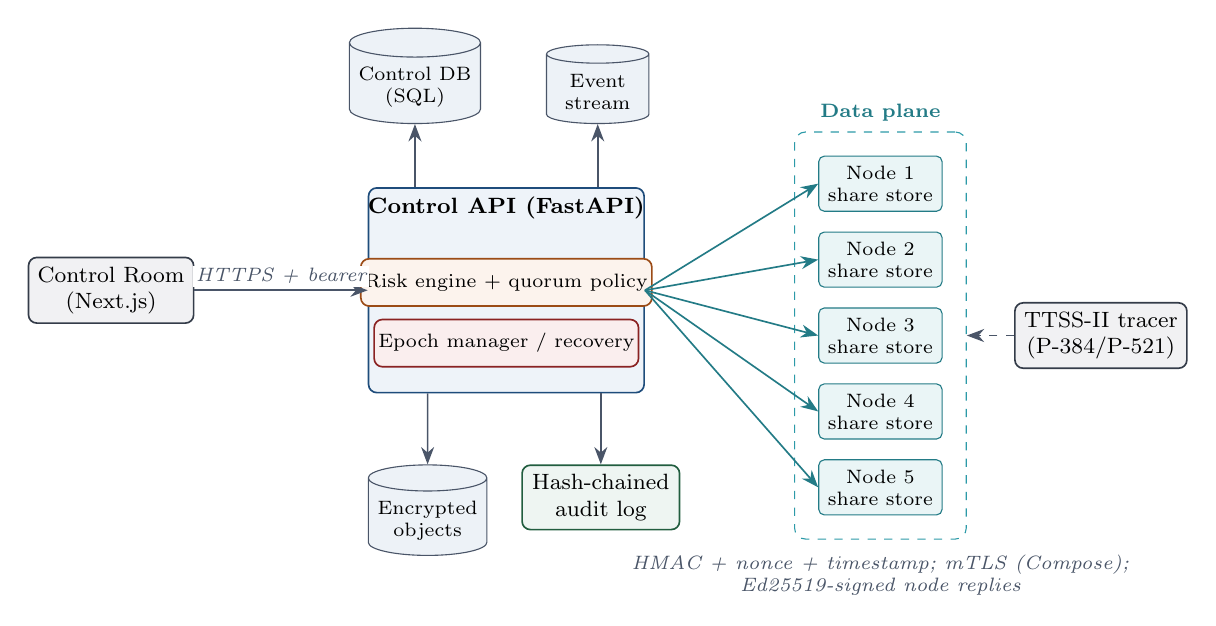
\begin{tikzpicture}[
  font=\footnotesize,
  box/.style={draw=#1!70!black, fill=#1!8, rounded corners=3pt, minimum height=8mm, minimum width=24mm, align=center, line width=0.6pt},
  box/.default=rsblue,
  db/.style={cylinder, shape border rotate=90, aspect=0.22, draw=rsgray, fill=rslight, minimum width=13mm, minimum height=10mm, align=center, font=\scriptsize},
  node/.style={draw=rsteal!80!black, fill=rsteal!10, rounded corners=2pt, minimum width=15mm, minimum height=7mm, align=center, font=\scriptsize},
  arr/.style={-{Stealth[length=2.2mm]}, line width=0.6pt, draw=rsgray},
  lbl/.style={font=\scriptsize\itshape, text=rsgray, fill=white, inner sep=1pt}
]
% users
\node[box=rsgray, minimum width=20mm] (ui) {Control Room\\(Next.js)};
\node[box=rsblue, right=22mm of ui, minimum width=35mm, minimum height=26mm, anchor=west, yshift=0mm] (api) {};
\node[font=\footnotesize\bfseries, anchor=north] at (api.north) {Control API (FastAPI)};
\node[box=rsorange, minimum width=28mm, minimum height=6mm, font=\scriptsize, inner sep=1.5pt] (risk) at ($(api.center)+(0,0.1)$) {Risk engine + quorum policy};
\node[box=rsred, minimum width=28mm, minimum height=6mm, font=\scriptsize, inner sep=1.5pt, below=1.5mm of risk] (epoch) {Epoch manager / recovery};
% stores
\node[db, above=8mm of api.north west, xshift=6mm] (pg) {Control DB\\(SQL)};
\node[db, above=8mm of api.north east, xshift=-6mm] (redis) {Event\\stream};
\node[db, below=9mm of api, xshift=-10mm] (obj) {Encrypted\\objects};
\node[box=rsgreen, below=9mm of api, xshift=12mm, minimum width=20mm] (audit) {Hash-chained\\audit log};
% nodes
\node[node, right=22mm of api.north east, anchor=north west, yshift=4mm] (n1) {Node 1\\share store};
\node[node, below=2.5mm of n1] (n2) {Node 2\\share store};
\node[node, below=2.5mm of n2] (n3) {Node 3\\share store};
\node[node, below=2.5mm of n3] (n4) {Node 4\\share store};
\node[node, below=2.5mm of n4] (n5) {Node 5\\share store};
\begin{scope}[on background layer]
  \node[draw=rsteal, dashed, rounded corners=4pt, fit=(n1)(n5), inner sep=3mm, label={[font=\scriptsize\bfseries, text=rsteal!80!black]above:Data plane}] (plane) {};
\end{scope}
% tracer
\node[box=rsgray, right=6mm of plane, minimum width=20mm] (tracer) {TTSS-II tracer\\(P-384/P-521)};
% edges
\draw[arr] (ui.east) -- node[lbl, above, yshift=1pt]{HTTPS + bearer} (api.west|-ui.east);
\draw[arr] ($(api.north west)+(6mm,0)$) -- (pg);
\draw[arr] ($(api.north east)+(-6mm,0)$) -- (redis);
\draw[arr] (obj|-api.south) -- (obj);
\draw[arr] (audit|-api.south) -- (audit);
\foreach \n in {n1,n2,n3,n4,n5} \draw[arr, rsteal!80!black] (api.east) -- (\n.west);
\node[lbl, align=center, below=1.5mm of plane] {HMAC + nonce + timestamp; mTLS (Compose);\\Ed25519-signed node replies};
\draw[arr, dashed] (tracer.west) -- (plane.east);
\end{tikzpicture}
\caption{\RS{} architecture. The control plane decides \emph{when} a new epoch is needed; the data plane stores exactly one share per node per generation. Node requests are HMAC-authenticated and replay-protected~\cite{rfc2104}, node responses are Ed25519-signed, and every state change is appended to a hash-chained audit log.}
\label{fig:arch}
\end{figure*}

\subsection{Adversary}
We consider an adversary that can compromise up to $c$ of the $n$ nodes and read their stored shares, and an environment in which up to $u$ nodes may be unavailable. Compromise is not directly observable; the system sees only \emph{signals} (failed authentication, invalid shares or signatures, missed heartbeats, abnormal request bursts, suspicious or failed recoveries). We assume the control plane and the recovery path are trusted during a recovery, that the epoch-transition code runs correctly, and that compromise of old shares after their epoch is retired does not compromise newer ciphertext. Rotation protects \emph{future} ciphertext only: it cannot revoke copies of old ciphertext and old keys an adversary already holds. We do not address a compromised control plane, side channels, or denial of service.

\subsection{Security goals}
\begin{itemize}
  \item \textbf{G1 Threshold integrity.} The active threshold of a vault always equals the threshold under which its current shares were generated.
  \item \textbf{G2 Fail-closed transitions.} A failed or partial transition never activates an incomplete share set; recovery is frozen until safety is re-established.
  \item \textbf{G3 Separation of duties.} Recovery requires a request and an approval by a different, administrator-role identity.
  \item \textbf{G4 Accountability.} Leaks can be investigated with TTSS-II tracing, and administrative actions are recorded in a tamper-evident log.
\end{itemize}

% ===========================================================================
\section{Risk Engine and Quorum Policy}
\label{sec:risk}

\subsection{Explainable risk score}
Each event $e$ has a kind $\kappa(e)$ with a fixed weight $w_{\kappa}$ (Table~\ref{tab:weights}), a target node $\nu(e)$ and a timestamp $\tau_e$. Its contribution decays linearly to zero over a window $D$ (24\,h by default):
\begin{equation}
  \rho_e(\tau) \;=\; \operatorname{round}\!\left( w_{\kappa(e)} \cdot \max\!\Bigl(0,\; 1 - \frac{\tau-\tau_e}{D}\Bigr) \right).
  \label{eq:decay}
\end{equation}
Per-node and overall scores are capped at 100:
\begin{align}
  R_i(\tau) &= \min\Bigl(100, \sum_{e:\,\nu(e)=i} \rho_e(\tau)\Bigr), \nonumber\\
  R(\tau) &= \min\Bigl(100, \sum_{i=1}^{n} R_i(\tau)\Bigr).
  \label{eq:score}
\end{align}
Events are de-duplicated by identifier. Because every point of $R$ can be attributed to a named event, the Control Room can show \emph{why} the threshold changed (Fig.~\ref{fig:ui}(b)).

\begin{table}[t]
\centering
\caption{Risk-event weights used by the engine.}
\label{tab:weights}
\begin{tabular}{@{}lr@{}}
\toprule
Event kind & Weight $w_\kappa$ \\
\midrule
Failed authentication            & 15 \\
Missed heartbeat                 & 15 \\
Failed recovery                  & 15 \\
Abnormal request burst           & 20 \\
Suspicious recovery              & 20 \\
Invalid share                    & 30 \\
Share integrity failure          & 30 \\
Invalid node signature           & 40 \\
\bottomrule
\end{tabular}
\end{table}

\subsection{Score-to-quorum mapping}
The policy maps the score to a target threshold
\begin{equation}
  t^\star(R) \;=\;
  \begin{cases}
    2, & 0 \le R < 30 \quad (\text{low}),\\
    3, & 30 \le R < 60 \quad (\text{medium}),\\
    4, & 60 \le R \le 100 \quad (\text{high}),
  \end{cases}
  \label{eq:policy}
\end{equation}
and a confirmed critical event forces $t^\star=4$. The bands are illustrated in Fig.~\ref{fig:bands}. Transitions are asymmetric. \emph{Escalation} ($t^\star > t$) is immediate and freezes recovery until the new epoch is active. \emph{De-escalation} ($t^\star < t$) requires administrator authorisation and a cooldown $\Delta$ (1\,h by default) measured from when the lower score was first observed; a renewed rise during the cooldown cancels it. This hysteresis prevents an adversary from forcing rapid re-keying by toggling signals, and prevents silent weakening.

\begin{figure}[t]
\centering
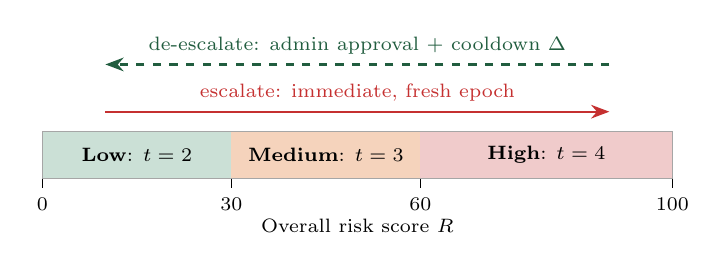
\begin{tikzpicture}[font=\scriptsize]
  \def\W{8.0}
  \fill[rsgreen!25]  (0,0) rectangle (0.30*\W,0.6);
  \fill[rsorange!30] (0.30*\W,0) rectangle (0.60*\W,0.6);
  \fill[rsred!25]    (0.60*\W,0) rectangle (\W,0.6);
  \draw[gray!70] (0,0) rectangle (\W,0.6);
  \node at (0.15*\W,0.3) {\textbf{Low}: $t=2$};
  \node at (0.45*\W,0.3) {\textbf{Medium}: $t=3$};
  \node at (0.80*\W,0.3) {\textbf{High}: $t=4$};
  \foreach \x/\l in {0/0,0.30/30,0.60/60,1/100} \draw (\x*\W,0) -- ++(0,-0.12) node[below]{\l};
  \node at (0.5*\W,-0.6) {Overall risk score $R$};
  \draw[-{Stealth}, rsred, thick] (0.1*\W,0.85) -- node[above]{escalate: immediate, fresh epoch} (0.9*\W,0.85);
  \draw[-{Stealth}, rsgreen!70!black, thick, dashed] (0.9*\W,1.45) -- node[above]{de-escalate: admin approval + cooldown $\Delta$} (0.1*\W,1.45);
\end{tikzpicture}
\caption{Risk bands of Eq.~\eqref{eq:policy} and the asymmetric transition rule.}
\label{fig:bands}
\end{figure}

% ===========================================================================
\section{Fresh Cryptographic Epochs}
\label{sec:epochs}

\subsection{Why relabelling is unsound}
A 2-of-$n$ Asmuth--Bloom share set satisfies~\eqref{eq:ab} for $t=2$. Any two of its shares reconstruct $y_1,y_2$ by~\eqref{eq:crt}, whatever threshold the application later claims. ``Raising'' the threshold of a stored share set therefore changes nothing for an adversary who already holds two shares. A stricter threshold must come from new randomness: a new secret, new components~\eqref{eq:additive}, new encodings~\eqref{eq:y1}--\eqref{eq:yj} and new moduli satisfying~\eqref{eq:ab} for the new $t$. Re-sharing the \emph{same} DEK would leave the old 2-of-$n$ shares valid for it, so \RS{} also replaces the DEK and re-encrypts.

\subsection{Epoch transition protocol}
An epoch $E=(\mathit{id}, t, \DEK, \mathit{ct}, \{\sigma_i\})$ binds a vault's ciphertext to one share generation. Algorithm~\ref{alg:epoch} gives the transition; Fig.~\ref{fig:epoch} shows the state machine. The ciphertext is authenticated with associated data
\begin{equation}
  \mathit{ct} = \Enc^{\mathrm{GCM}}_{\DEK'}\bigl(N,\; P,\; \mathsf{AAD}=(\mathit{vault},\mathit{epoch},\mathit{ver})\bigr),
  \label{eq:gcm}
\end{equation}
so a ciphertext cannot be replayed into another vault or epoch without failing authentication. The 32-byte DEK is converted to an integer $s<2^{256}$ in fixed-width big-endian form before sharing.

\begin{algorithm}[t]
\caption{Risk-triggered epoch transition}
\label{alg:epoch}
\begin{algorithmic}[1]
\Require vault $v$ with active epoch $E$ (threshold $t$); risk score $R$
\State $t^\star \gets t^\star(R)$ \Comment{Eq.~\eqref{eq:policy}}
\If{$t^\star = t$} \Return $E$ \EndIf
\If{$t^\star < t$ \textbf{and} (not admin-approved \textbf{or} cooldown not elapsed)}
   \State \Return $E$ \Comment{de-escalation is gated}
\EndIf
\State freeze recovery for $v$; log \texttt{started}
\State $P \gets \Dec_{E.\DEK}(E.\mathit{ct})$ \Comment{restricted worker}
\State $\DEK' \xleftarrow{\$} \{0,1\}^{256}$;\; $\mathit{id}' \gets$ fresh epoch id
\State $\mathit{ct}' \gets \Enc_{\DEK'}(P;\,v,\mathit{id}',\mathit{ver})$ \Comment{Eq.~\eqref{eq:gcm}}
\State $(\{\sigma'_i\}, \mathsf{tk}, \mathsf{vk}) \gets \textsc{ShareII}(\mathrm{int}(\DEK'), n, t^\star)$
\ForAll{nodes $i$}
   \State send $\sigma'_i$ (HMAC, nonce, timestamp); await signed ack
\EndFor
\If{all $n$ acks valid}
   \State atomically: $E.\mathit{status}\gets$ \textsc{retired};\; activate $E'$
   \State unfreeze recovery; log \texttt{completed}
   \State \Return $E'$
\Else
   \State keep $E$ active, keep recovery frozen \Comment{fail closed}
   \State log \texttt{failed}; \Return $E$
\EndIf
\end{algorithmic}
\end{algorithm}

\begin{figure}[t]
\centering
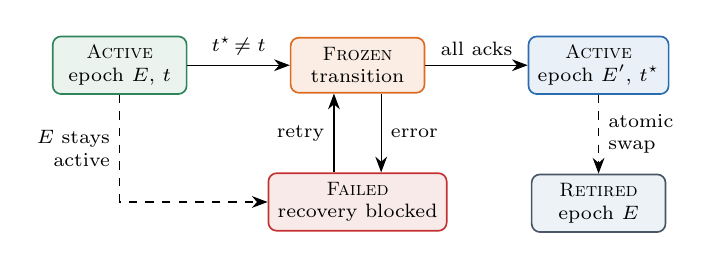
\begin{tikzpicture}[
  font=\scriptsize, >={Stealth[length=2mm]},
  st/.style={draw, rounded corners=3pt, minimum width=17mm, minimum height=7mm, align=center, line width=0.6pt},
]
\node[st, draw=rsgreen, fill=rsgreen!10] (act) {\textsc{Active}\\epoch $E$, $t$};
\node[st, draw=rsorange, fill=rsorange!12, right=13mm of act] (fr) {\textsc{Frozen}\\transition};
\node[st, draw=rsblue, fill=rsblue!10, right=13mm of fr] (new) {\textsc{Active}\\epoch $E'$, $t^\star$};
\node[st, draw=rsgray, fill=rslight, below=10mm of new] (ret) {\textsc{Retired}\\epoch $E$};
\node[st, draw=rsred, fill=rsred!10, below=10mm of fr] (fail) {\textsc{Failed}\\recovery blocked};
\draw[->] (act) -- node[above]{$t^\star\!\neq t$} (fr);
\draw[->] (fr) -- node[above]{all acks} (new);
\draw[->] ($(fr.south)+(0.3,0)$) -- node[right]{error} ($(fail.north)+(0.3,0)$);
\draw[->] ($(fail.north)+(-0.3,0)$) -- node[left]{retry} ($(fr.south)+(-0.3,0)$);
\draw[->, dashed] (new) -- node[right, align=left]{atomic\\swap} (ret);
\draw[->, dashed] (act.south) |- node[pos=0.25, left, align=right]{$E$ stays\\active} (fail.west);
\end{tikzpicture}
\caption{Epoch life cycle. Activation is atomic; any failure leaves the previous epoch in place with recovery frozen, never a partially distributed share set.}
\label{fig:epoch}
\end{figure}

\begin{proposition}[Threshold integrity]
If every activated epoch is produced by Algorithm~\ref{alg:epoch}, then for every vault the active threshold equals the threshold under which its active shares were generated, and any shares from earlier epochs reconstruct only a retired DEK.
\end{proposition}
\begin{proof}[Sketch]
Activation happens only in the success branch, after $\textsc{ShareII}$ has generated $\{\sigma'_i\}$ for $t^\star$ and the epoch record stores $t^\star$; activation and retirement are a single transaction. $\DEK'$ is sampled independently of $E.\DEK$, so earlier shares, which encode $E.\DEK$ by~\eqref{eq:rec}, carry no information about $\DEK'$ beyond what the adversary could already learn from $P$.
\end{proof}

\subsection{Recovery}
A recovery request names a vault and records the active epoch and required share count $t$. A \emph{different} administrator must approve it (G3). The orchestrator then asks nodes for their shares using short-lived release tokens, verifies each signed response, reconstructs the DEK from the first $t$ valid shares via~\eqref{eq:crt}--\eqref{eq:rec}, decrypts and returns the file to the approver. Recovery is refused while a transition is frozen or when fewer than $t$ valid shares are obtained.

% ===========================================================================
\section{Implementation}
\label{sec:impl}

\RS{} is about 3{,}500 lines of Python~3.11+ (excluding tests) plus a TypeScript dashboard. Table~\ref{tab:impl} summarises the components.

\begin{table}[t]
\centering
\caption{Implementation components.}
\label{tab:impl}
\setlength{\tabcolsep}{4pt}
\begin{tabular}{@{}p{0.29\columnwidth}p{0.63\columnwidth}@{}}
\toprule
Component & Realisation \\
\midrule
ABSS-I/II & CSPRNG-driven Miller--Rabin primes~\cite{rabin1980primality}; $m_0$ sized to $|s|+64$ bits of headroom; strict check of~\eqref{eq:ab}; CRT reconstruction with range and consistency checks \\
TTSS-I/II & Black-box tracing (Eq.~\eqref{eq:trace}) with a query budget; TTSS-II commitments on secp384r1/secp521r1~\cite{sec2v2} via PyCA/OpenSSL \\
Encryption & AES-256-GCM, 96-bit nonce, AAD $=$ (vault, epoch, version)~\cite{dworkin2007gcm} \\
Node plane & 5 node agents, separate SQLite stores; HMAC-SHA256 requests with timestamp ($\pm30$\,s) and nonce~\cite{rfc2104}; Ed25519-signed responses; mTLS in the Compose deployment \\
Audit & SHA-256 hash chain over canonical JSON records (Eq.~\eqref{eq:audit})~\cite{schneier1999audit,crosby2009tamper} \\
Control plane & FastAPI, SQLAlchemy/Alembic, optional Redis Streams, WebSocket events, role-based auth, rate limiting \\
Interface & Next.js Control Room (Fig.~\ref{fig:ui}) \\
Tests & 34 tests (pytest, Hypothesis~\cite{maciver2019hypothesis}): subset reconstruction properties, crypto units, API flows, node authorisation, offline nodes, tracing, audit, certificates \\
\bottomrule
\end{tabular}
\end{table}

\paragraph*{Parameter generation} The default $m_0$ is the next prime above $2^{|s|+64}$ rather than just above $s$, so that $m_0$ does not reveal how close the secret lies to a public bound. Share moduli are consecutive primes above $m_0 2^{t+1}$, extended until~\eqref{eq:ab} holds. For a 256-bit DEK this gives $m_0\approx 2^{320}$; each share holds $t$ residues, so total share storage grows linearly in $t$ (Table~\ref{tab:costs}).

\paragraph*{Tracing group} The paper writes its group multiplicatively; we use additive notation on standardised prime-order curves, choosing P-384 when $m_n<q_{384}$ and P-521 otherwise, and reject parameters with $q \le m_n$.

\paragraph*{Audit chain} Record $k$ with sequence number $k$, timestamp $\tau_k$, type, actor and payload is linked as
\begin{equation}
  h_k = \mathrm{SHA256}\bigl(\mathrm{canon}(k, \tau_k, \mathit{type}_k, \mathit{actor}_k, \mathit{payload}_k, h_{k-1})\bigr),
  \label{eq:audit}
\end{equation}
with $h_0 = 0^{256}$. Verification recomputes every $h_k$ and checks the links; any change to a stored record breaks the chain from that point~\cite{crosby2009tamper}.

% ===========================================================================
\section{Evaluation}
\label{sec:eval}

\subsection{Methodology}
The experiment runner calls the real cryptographic modules. For each of $T=5$ trials it creates a fresh random 256-bit secret and a TTSS-II share generation for each $t\in\{2,3,4\}$ with $n=5$, and times one complete rotation (decrypt, new DEK, re-encrypt, re-share) per threshold. It then evaluates a $5\times5$ grid of scenarios with $u\in\{0,\dots,4\}$ unavailable nodes and $c\in\{0,\dots,4\}$ compromised nodes under four policies: fixed 2-, 3- and 4-of-5, and risk-adaptive. In each scenario:
\begin{itemize}
  \item \emph{legitimate recovery} succeeds iff $n-u \ge t$, and is checked by actually reconstructing and comparing the secret;
  \item \emph{attacker reconstruction} succeeds iff the $c$ compromised nodes hold at least $t$ shares, and is checked by actually reconstructing from those shares;
  \item if $1\le \min(c, t-1)$, a reconstruction box embedding $\min(c,t-1)$ shares is traced with TTSS-II (at most 64 queries) and the accusation is checked.
\end{itemize}
For the adaptive policy the scenario's detector produces
\begin{equation}
  R_{\text{scen}} = \min(100,\; 20c + 15u),
  \label{eq:scen}
\end{equation}
i.e.\ one ``suspicious recovery'' signal per compromised node and one ``missed heartbeat'' per unavailable node, and the threshold follows~\eqref{eq:policy}. This yields $4\times 25\times 5 = 500$ rows. Timings were taken on a single development workstation (Python~3.13, OpenSSL via PyCA).

\emph{Caveat.} Equation~\eqref{eq:scen} gives the detector perfect knowledge of $c$. Rates in this section are therefore \emph{fractions of scripted scenarios}, not probabilities of real-world compromise, and they show the best case for adaptivity. Section~\ref{sec:analytic} adds an analytical model, and Section~\ref{sec:limits} discusses the gap.

\subsection{Security--availability trade-off}
Table~\ref{tab:summary} and Fig.~\ref{fig:rates} summarise the results. Raising a fixed threshold lowers the scripted attacker success rate by 20 percentage points per step and lowers legitimate recovery by the same amount. The adaptive policy reaches the \emph{same} attacker rate as fixed 4-of-5 (20\%) while recovering in 48\% of scenarios, 8 points more than fixed 4-of-5. Fig.~\ref{fig:tradeoff} places the four policies on the trade-off plane: the three fixed policies lie on one line, and the adaptive policy lies above it.

\begin{table}[t]
\centering
\caption{Scenario outcomes per policy (125 scenarios each, 5 trials). Times are means $\pm$ standard deviation.}
\label{tab:summary}
\setlength{\tabcolsep}{3.5pt}
\begin{tabular}{@{}lcccc@{}}
\toprule
Policy & Recovery & Attacker & Share gen. & Reconstr. \\
       & success  & reconstr. & (ms) & (ms) \\
\midrule
Fixed 2-of-5   & 80\% & 60\% & $73.3\pm 9.6$  & $4.15\pm1.56$ \\
Fixed 3-of-5   & 60\% & 40\% & $82.0\pm 19.9$ & $4.14\pm0.66$ \\
Fixed 4-of-5   & 40\% & 20\% & $58.0\pm 2.8$  & $4.26\pm1.20$ \\
\textbf{Risk-adaptive} & \textbf{48\%} & \textbf{20\%} & $65.6\pm 14.9$ & $4.11\pm0.49$ \\
\bottomrule
\end{tabular}
\end{table}

\begin{figure}[t]
\centering
\begin{tikzpicture}
\begin{axis}[rsaxis,
  width=\columnwidth, height=5.0cm,
  ybar=1.5pt, bar width=9pt,
  ymin=0, ymax=100, ylabel={Scenarios (\%)},
  symbolic x coords={Fixed2,Fixed3,Fixed4,Adaptive},
  xtick=data,
  xticklabels={Fixed 2-of-5, Fixed 3-of-5, Fixed 4-of-5, Adaptive},
  x tick label style={font=\scriptsize},
  enlarge x limits=0.18,
  nodes near coords, nodes near coords style={font=\tiny},
  legend pos=north east, legend columns=1,
]
\addplot[fill=rsteal, draw=rsteal!70!black] table[x=policy, y=recovery]{data/policy_summary.dat};
\addplot[fill=rsred!70, draw=rsred!80!black] table[x=policy, y=attacker]{data/policy_summary.dat};
\legend{Legitimate recovery, Attacker reconstruction}
\end{axis}
\end{tikzpicture}
\caption{Legitimate-recovery and scripted attacker-reconstruction rates over the $5\times5$ scenario grid. Adaptive matches fixed 4-of-5 on attacker reconstruction with higher availability.}
\label{fig:rates}
\end{figure}

\begin{figure}[t]
\centering
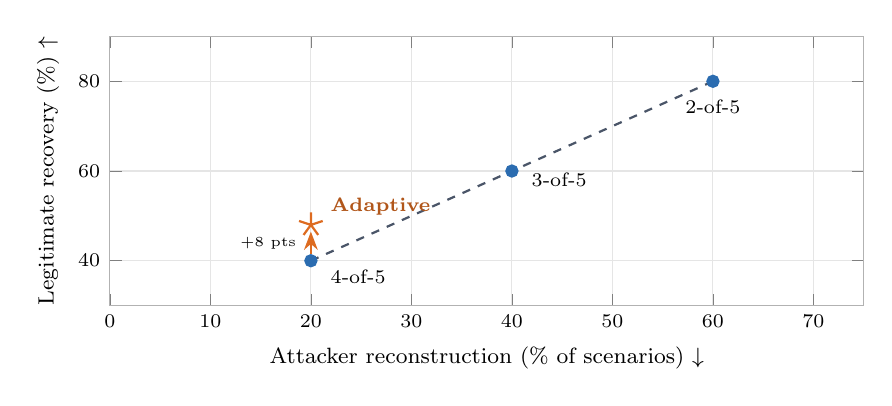
\begin{tikzpicture}
\begin{axis}[rsaxis,
  width=0.92\columnwidth, height=5.0cm,
  xmin=0, xmax=75, ymin=30, ymax=90,
  xlabel={Attacker reconstruction (\% of scenarios) $\downarrow$},
  ylabel={Legitimate recovery (\%) $\uparrow$},
]
\addplot[rsgray, dashed, thick, mark=*, mark options={fill=rsblue, draw=rsblue, solid}] coordinates {(20,40) (40,60) (60,80)};
\node[font=\scriptsize, anchor=north] at (axis cs:60,78) {2-of-5};
\node[font=\scriptsize, anchor=west] at (axis cs:41,58) {3-of-5};
\node[font=\scriptsize, anchor=north west] at (axis cs:21,40) {4-of-5};
\addplot[only marks, mark=star, mark size=4.5pt, rsorange, thick] coordinates {(20,48)};
\node[font=\scriptsize\bfseries, text=rsorange!80!black, anchor=south west] at (axis cs:21,48) {Adaptive};
\draw[-{Stealth}, rsorange, thick] (axis cs:20,41.5) -- (axis cs:20,46.5);
\node[font=\tiny, anchor=east] at (axis cs:19.5,44) {+8 pts};
\end{axis}
\end{tikzpicture}
\caption{Trade-off plane. The fixed thresholds lie on a straight frontier; the adaptive policy sits above it at the same attacker rate as 4-of-5.}
\label{fig:tradeoff}
\end{figure}

Fig.~\ref{fig:grid} explains the gain. The adaptive policy uses the lenient 2-of-5 threshold only when signals are weak ($R<30$), where no scripted adversary holds two shares. It moves to 3- or 4-of-5 as $c$ grows. The extra recoveries come from the cells $(u{=}2, c{\in}\{0,1\})$, where 3-of-5 still suffices with three nodes online and fixed 4-of-5 would refuse. The remaining attacker successes are the column $c=4$: with $n=5$ and a maximum profile of $t=4$, no policy can stop four colluding nodes, which argues for a $t=n$ or ``freeze'' profile at the top of the scale.

\begin{figure}[t]
\centering
\begin{tikzpicture}
\begin{axis}[
  width=0.82\columnwidth, height=0.82\columnwidth,
  enlargelimits=false,
  xmin=-0.5, xmax=4.5, ymin=-0.5, ymax=4.5,
  xtick={0,...,4}, ytick={0,...,4},
  xlabel={Compromised nodes $c$}, ylabel={Unavailable nodes $u$},
  tick label style={font=\scriptsize}, label style={font=\footnotesize},
  colormap={rs}{rgb255(0cm)=(198,239,206); rgb255(1cm)=(254,215,170); rgb255(2cm)=(254,178,178)},
  point meta min=2, point meta max=4,
  colorbar, colorbar style={ytick={2,3,4}, yticklabel style={font=\scriptsize}, ylabel={adaptive $t$}, ylabel style={font=\scriptsize}, width=2.5mm},
  axis on top,
]
\addplot[matrix plot*, mesh/cols=5, point meta=explicit,
  nodes near coords={\pgfmathprintnumber{\pgfplotspointmeta}},
  nodes near coords style={font=\scriptsize\bfseries, anchor=center, yshift=2pt},
] table[x=c, y=u, meta=t]{data/adaptive_grid.dat};
\addplot[only marks, mark=x, mark size=2.6pt, thick, rsgray] table[x expr=\thisrow{c}+0.28, y expr=\thisrow{u}-0.28]{data/grid_norecovery.dat};
\addplot[only marks, mark=triangle*, mark size=2.4pt, rsred] table[x expr=\thisrow{c}-0.28, y expr=\thisrow{u}-0.28]{data/grid_attacker.dat};
\end{axis}
\end{tikzpicture}
\caption{Threshold selected by the adaptive policy for each scenario (cell number). $\times$: legitimate recovery impossible ($n-u<t$); {\color{rsred}$\blacktriangle$}: scripted attacker reconstructs.}
\label{fig:grid}
\end{figure}

\subsection{Computational cost}
Table~\ref{tab:costs} and Fig.~\ref{fig:costs} report costs per threshold. Reconstruction ($t$ CRT solves) takes about 4.1--4.3\,ms and is essentially independent of $t$ at these sizes. Share generation (58--82\,ms) is dominated by probable-prime search and varies more from trial to trial (Fig.~\ref{fig:pertrial}) than between thresholds, so five trials cannot rank thresholds by generation cost. A complete rotation, the price of one adaptive escalation, took 60--67\,ms. Share storage grows linearly in $t$: 610, 817 and 1024 bytes for all five shares. Tracing correctly identified the embedded nodes in \textbf{60 of 60} distinct trace cases, in 26--38\,ms on average.

\begin{table}[t]
\centering
\caption{Cost per threshold over 5 trials (fixed policies).}
\label{tab:costs}
\setlength{\tabcolsep}{3pt}
\begin{tabular}{@{}ccccccc@{}}
\toprule
$t$ & Gen.\ (ms) & Rotation (ms) & Rec.\ (ms) & Bytes & Trace (ms) & Traced \\
\midrule
2 & $73.3\pm10.7$ & $59.6\pm3.5$  & $4.15$ & 610  & $26.5\pm10.7$ & 20/20 \\
3 & $82.0\pm22.1$ & $66.7\pm15.0$ & $4.14$ & 817  & $27.7\pm10.3$ & 20/20 \\
4 & $58.0\pm3.1$  & $63.5\pm10.3$ & $4.26$ & 1024 & $38.1\pm16.6$ & 20/20 \\
\bottomrule
\end{tabular}
\end{table}

\begin{figure}[t]
\centering
\begin{tikzpicture}
\begin{axis}[rsaxis,
  width=\columnwidth, height=5.0cm,
  ybar=1pt, bar width=7pt,
  ymin=0, ymax=110, ylabel={Time (ms)},
  xtick={2,3,4}, xticklabels={2-of-5, 3-of-5, 4-of-5},
  xlabel={Threshold}, enlarge x limits=0.25,
  legend style={at={(0.5,1.03)}, anchor=south}, legend columns=4,
  error bars/y dir=both, error bars/y explicit,
]
\addplot[fill=rsblue!70, draw=rsblue!80!black, error bars/.cd, y dir=both, y explicit] table[x=t, y=gen, y error=gensd]{data/threshold_costs.dat};
\addplot[fill=rsorange!70, draw=rsorange!80!black, error bars/.cd, y dir=both, y explicit] table[x=t, y=rot, y error=rotsd]{data/threshold_costs.dat};
\addplot[fill=rsgreen!60, draw=rsgreen!80!black, error bars/.cd, y dir=both, y explicit] table[x=t, y=trace, y error=tracesd]{data/threshold_costs.dat};
\addplot[fill=rsgray!50, draw=rsgray] table[x=t, y=rec]{data/threshold_costs.dat};
\legend{Share generation, Full rotation, TTSS-II trace, Reconstruction}
\end{axis}
\end{tikzpicture}
\caption{Mean cost per operation ($\pm1$ s.d.). Reconstruction is about 4\,ms at all thresholds.}
\label{fig:costs}
\end{figure}

\begin{figure}[t]
\centering
\begin{tikzpicture}
\begin{axis}[rsaxis,
  width=\columnwidth, height=4.3cm,
  xlabel={Trial}, ylabel={Share gen.\ (ms)},
  xtick={1,...,5}, ymin=40, ymax=110,
  legend style={at={(0.5,1.03)}, anchor=south}, legend columns=3,
]
\addplot[rsblue, thick, mark=*] table[x=trial, y=t2]{data/per_trial_generation.dat};
\addplot[rsorange, thick, mark=square*] table[x=trial, y=t3]{data/per_trial_generation.dat};
\addplot[rsred, thick, mark=triangle*] table[x=trial, y=t4]{data/per_trial_generation.dat};
\legend{$t=2$, $t=3$, $t=4$}
\end{axis}
\end{tikzpicture}
\caption{Per-trial TTSS-II share-generation time. Variation between trials (random prime search) is larger than variation between thresholds.}
\label{fig:pertrial}
\end{figure}

\subsection{Analytical model}
\label{sec:analytic}
To see the measured rates as points on a continuum, assume that each node is compromised independently with probability $p$ and online independently with probability $a$. Then
\begin{align}
  P_{\text{att}}(t;p) &= \sum_{k=t}^{n} \binom{n}{k} p^{k} (1-p)^{n-k}, \label{eq:patt}\\
  P_{\text{rec}}(t;a) &= \sum_{k=t}^{n} \binom{n}{k} a^{k} (1-a)^{n-k}. \label{eq:prec}
\end{align}
Fig.~\ref{fig:analytic} plots~\eqref{eq:patt}--\eqref{eq:prec} for $n=5$. At $p=0.1$, moving from $t=2$ to $t=4$ reduces $P_{\text{att}}$ from $0.081$ to $4.6\times10^{-4}$, while at $a=0.9$ it reduces $P_{\text{rec}}$ only from $0.9995$ to $0.919$. The cost of a strict threshold is paid mainly when availability is poor. A risk-adaptive policy aims to pay that cost only when compromise is likely; how well it succeeds depends on how well the signals track $p$.

\begin{figure}[t]
\centering
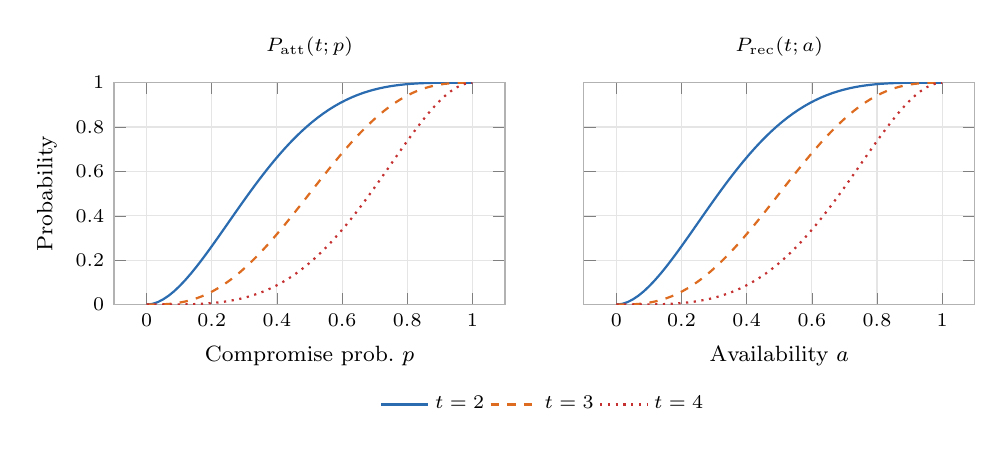
\begin{tikzpicture}
\begin{groupplot}[group style={group size=2 by 1, horizontal sep=10mm},
  rsaxis, width=0.54\columnwidth, height=4.4cm, domain=0:1, samples=60, ymin=0, ymax=1]
\nextgroupplot[xlabel={Compromise prob.\ $p$}, ylabel={Probability}, title={\scriptsize $P_{\text{att}}(t;p)$}, legend to name=anlegend, legend columns=3]
\addplot[rsblue, thick] {1-(1-x)^5-5*x*(1-x)^4};
\addplot[rsorange, thick, dashed] {10*x^3*(1-x)^2+5*x^4*(1-x)+x^5};
\addplot[rsred, thick, dotted] {5*x^4*(1-x)+x^5};
\legend{$t=2$, $t=3$, $t=4$}
\nextgroupplot[xlabel={Availability $a$}, title={\scriptsize $P_{\text{rec}}(t;a)$}, yticklabels={}]
\addplot[rsblue, thick] {1-(1-x)^5-5*x*(1-x)^4};
\addplot[rsorange, thick, dashed] {10*x^3*(1-x)^2+5*x^4*(1-x)+x^5};
\addplot[rsred, thick, dotted] {5*x^4*(1-x)+x^5};
\end{groupplot}
\node[below=9mm] at ($(group c1r1.south)!0.5!(group c2r1.south)$) {\pgfplotslegendfromname{anlegend}};
\end{tikzpicture}
\caption{Binomial model of Eqs.~\eqref{eq:patt}--\eqref{eq:prec} for $n=5$ (analytical, not measured). The two panels share one functional form, so a higher threshold moves both curves to the right.}
\label{fig:analytic}
\end{figure}

\subsection{End-to-end demonstration}
We ran the full stack locally (five node stores, SQLite control database) and drove it through the API. Two vaults were initialised at 2-of-5, each requiring acknowledgements from all five nodes. A simulated failed authentication on node~2 raised $R$ to 15 (low; no change). A simulated invalid share on node~4 added 30, giving $R=45$ (medium). The engine then rotated \emph{both} vaults to fresh 3-of-5 epochs and retired the 2-of-5 epochs, while all nodes remained online. A TTSS-II investigation with node~1's share embedded in a box identified node~1 and passed public verification. A subsequent recovery request recorded that 3 shares were required. Fig.~\ref{fig:ui} shows the resulting Control Room views.

\begin{figure*}[t]
\centering
\subfloat[Overview: risk 45 (medium), active quorum 3-of-5, node topology and recent audit events.]{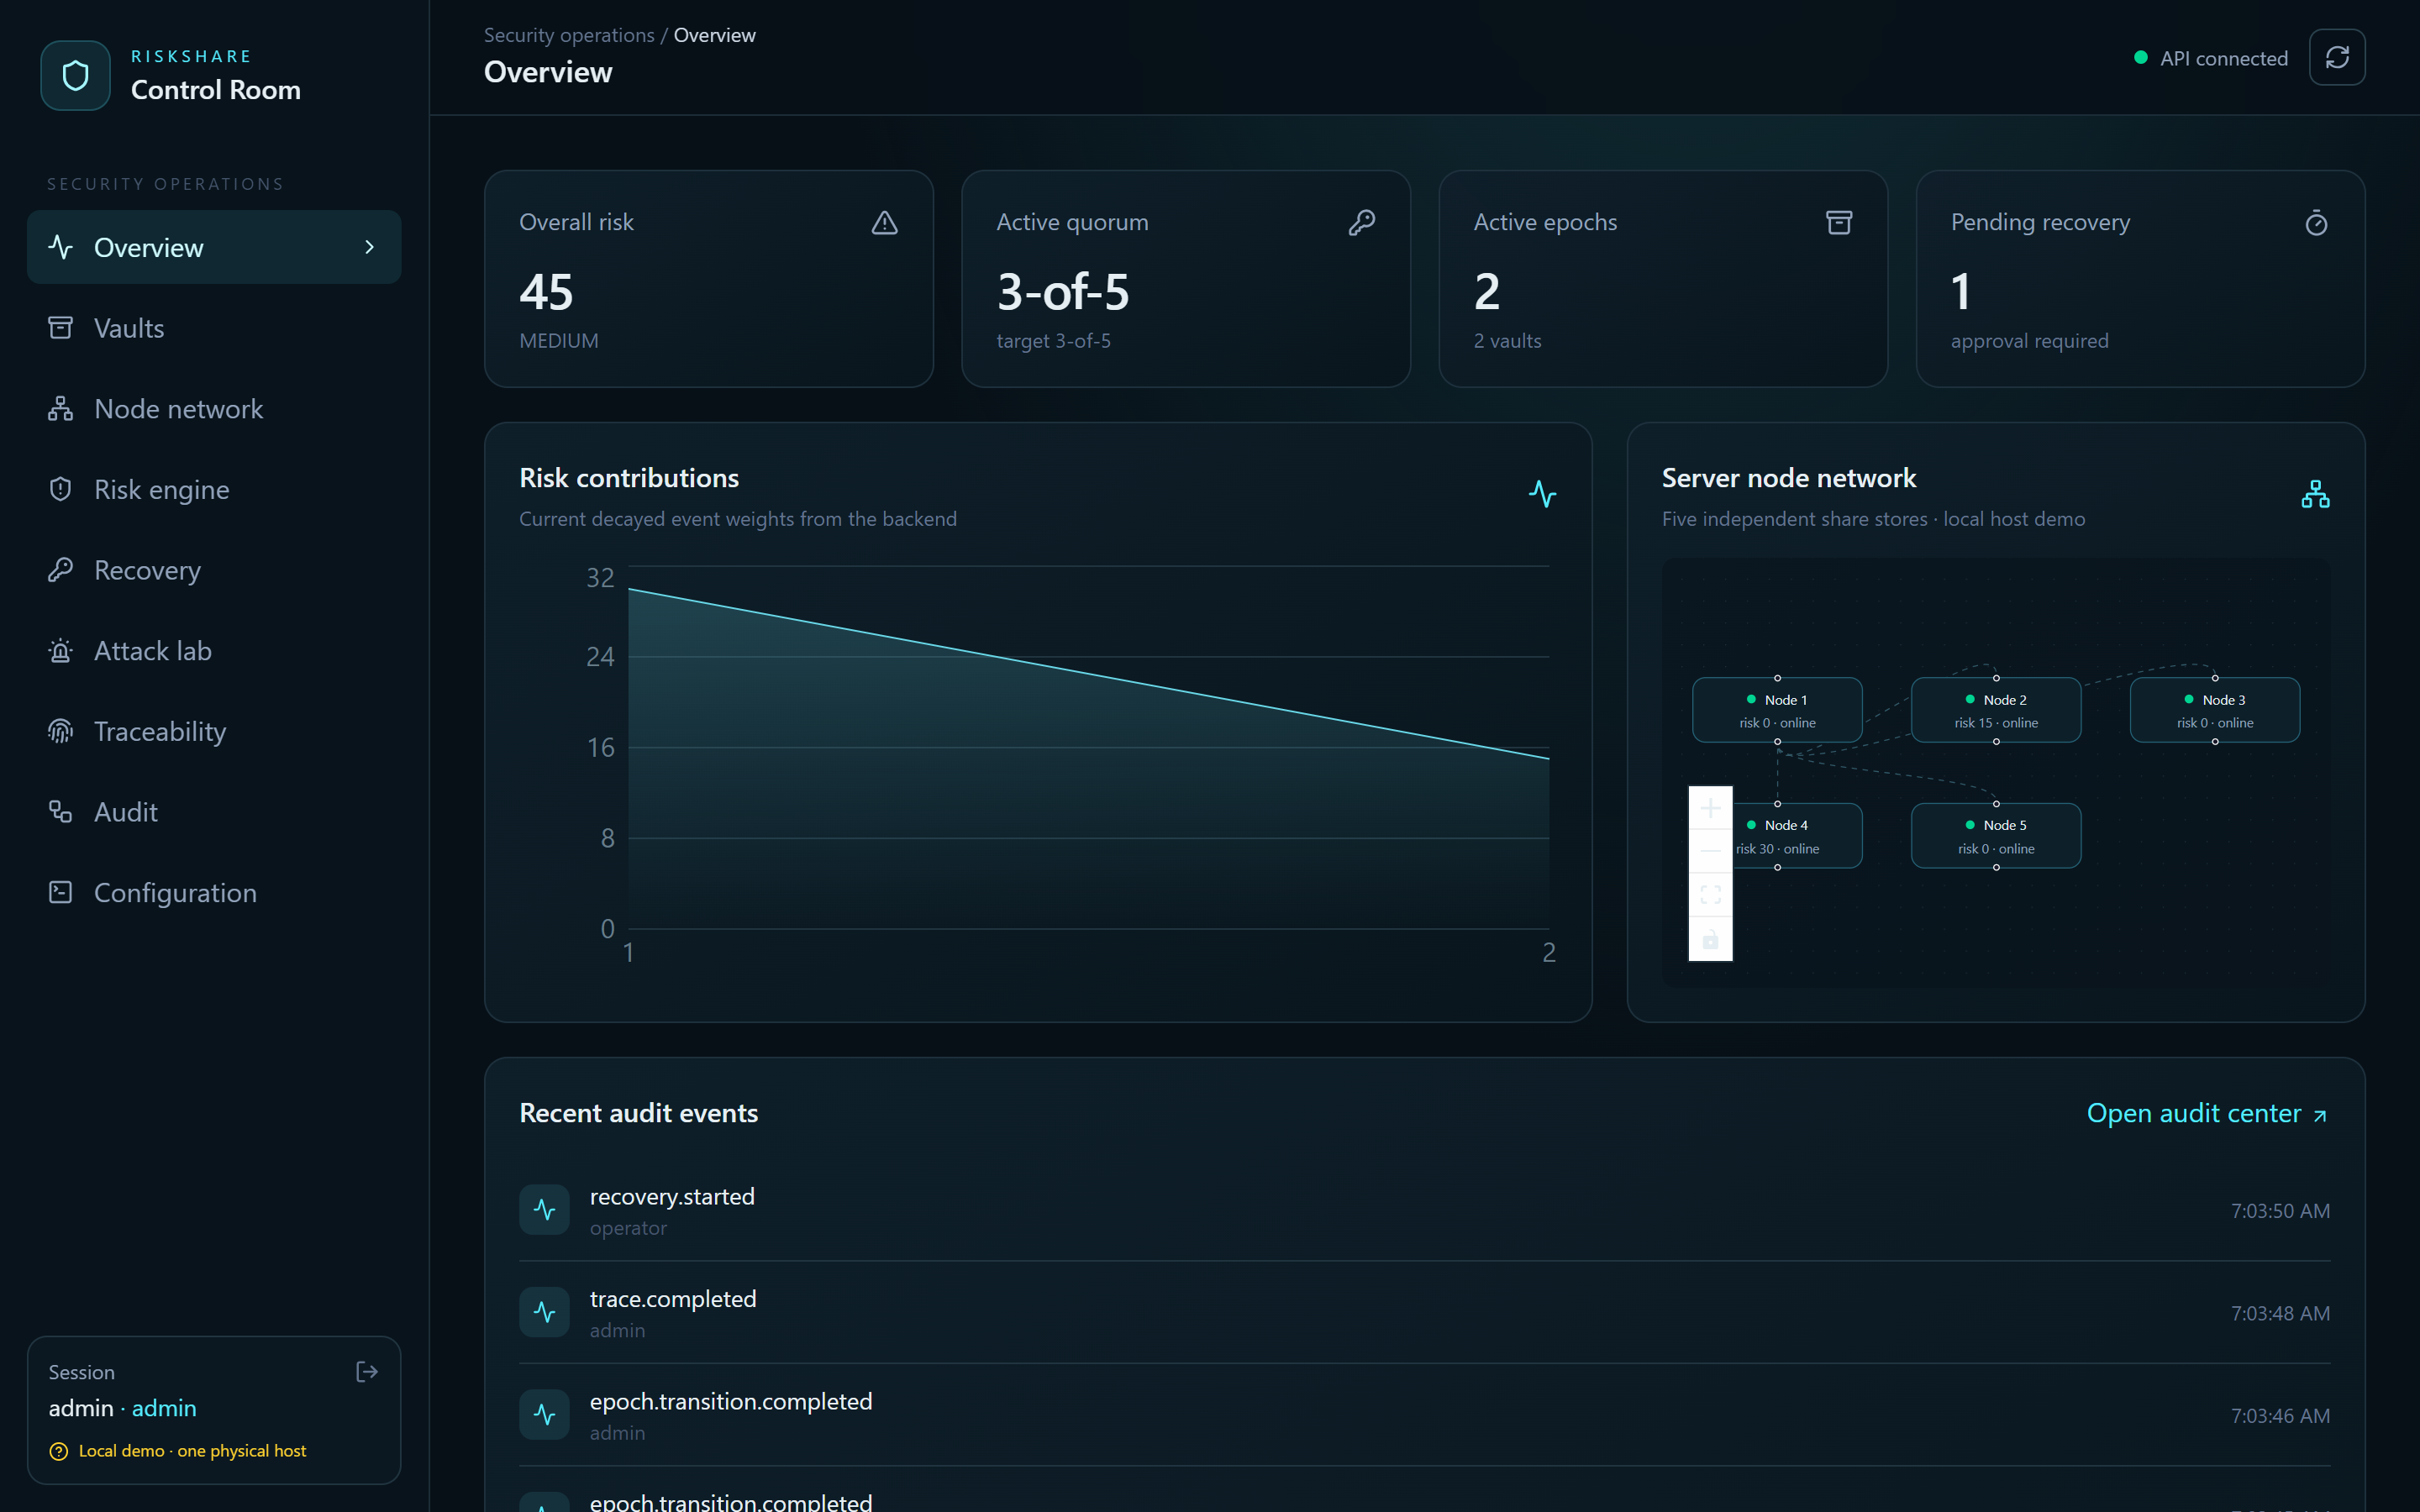
\includegraphics[width=0.485\textwidth]{figures/ui-overview.png}}\hfill
\subfloat[Risk engine: per-event explanation of the score and the policy bands.]{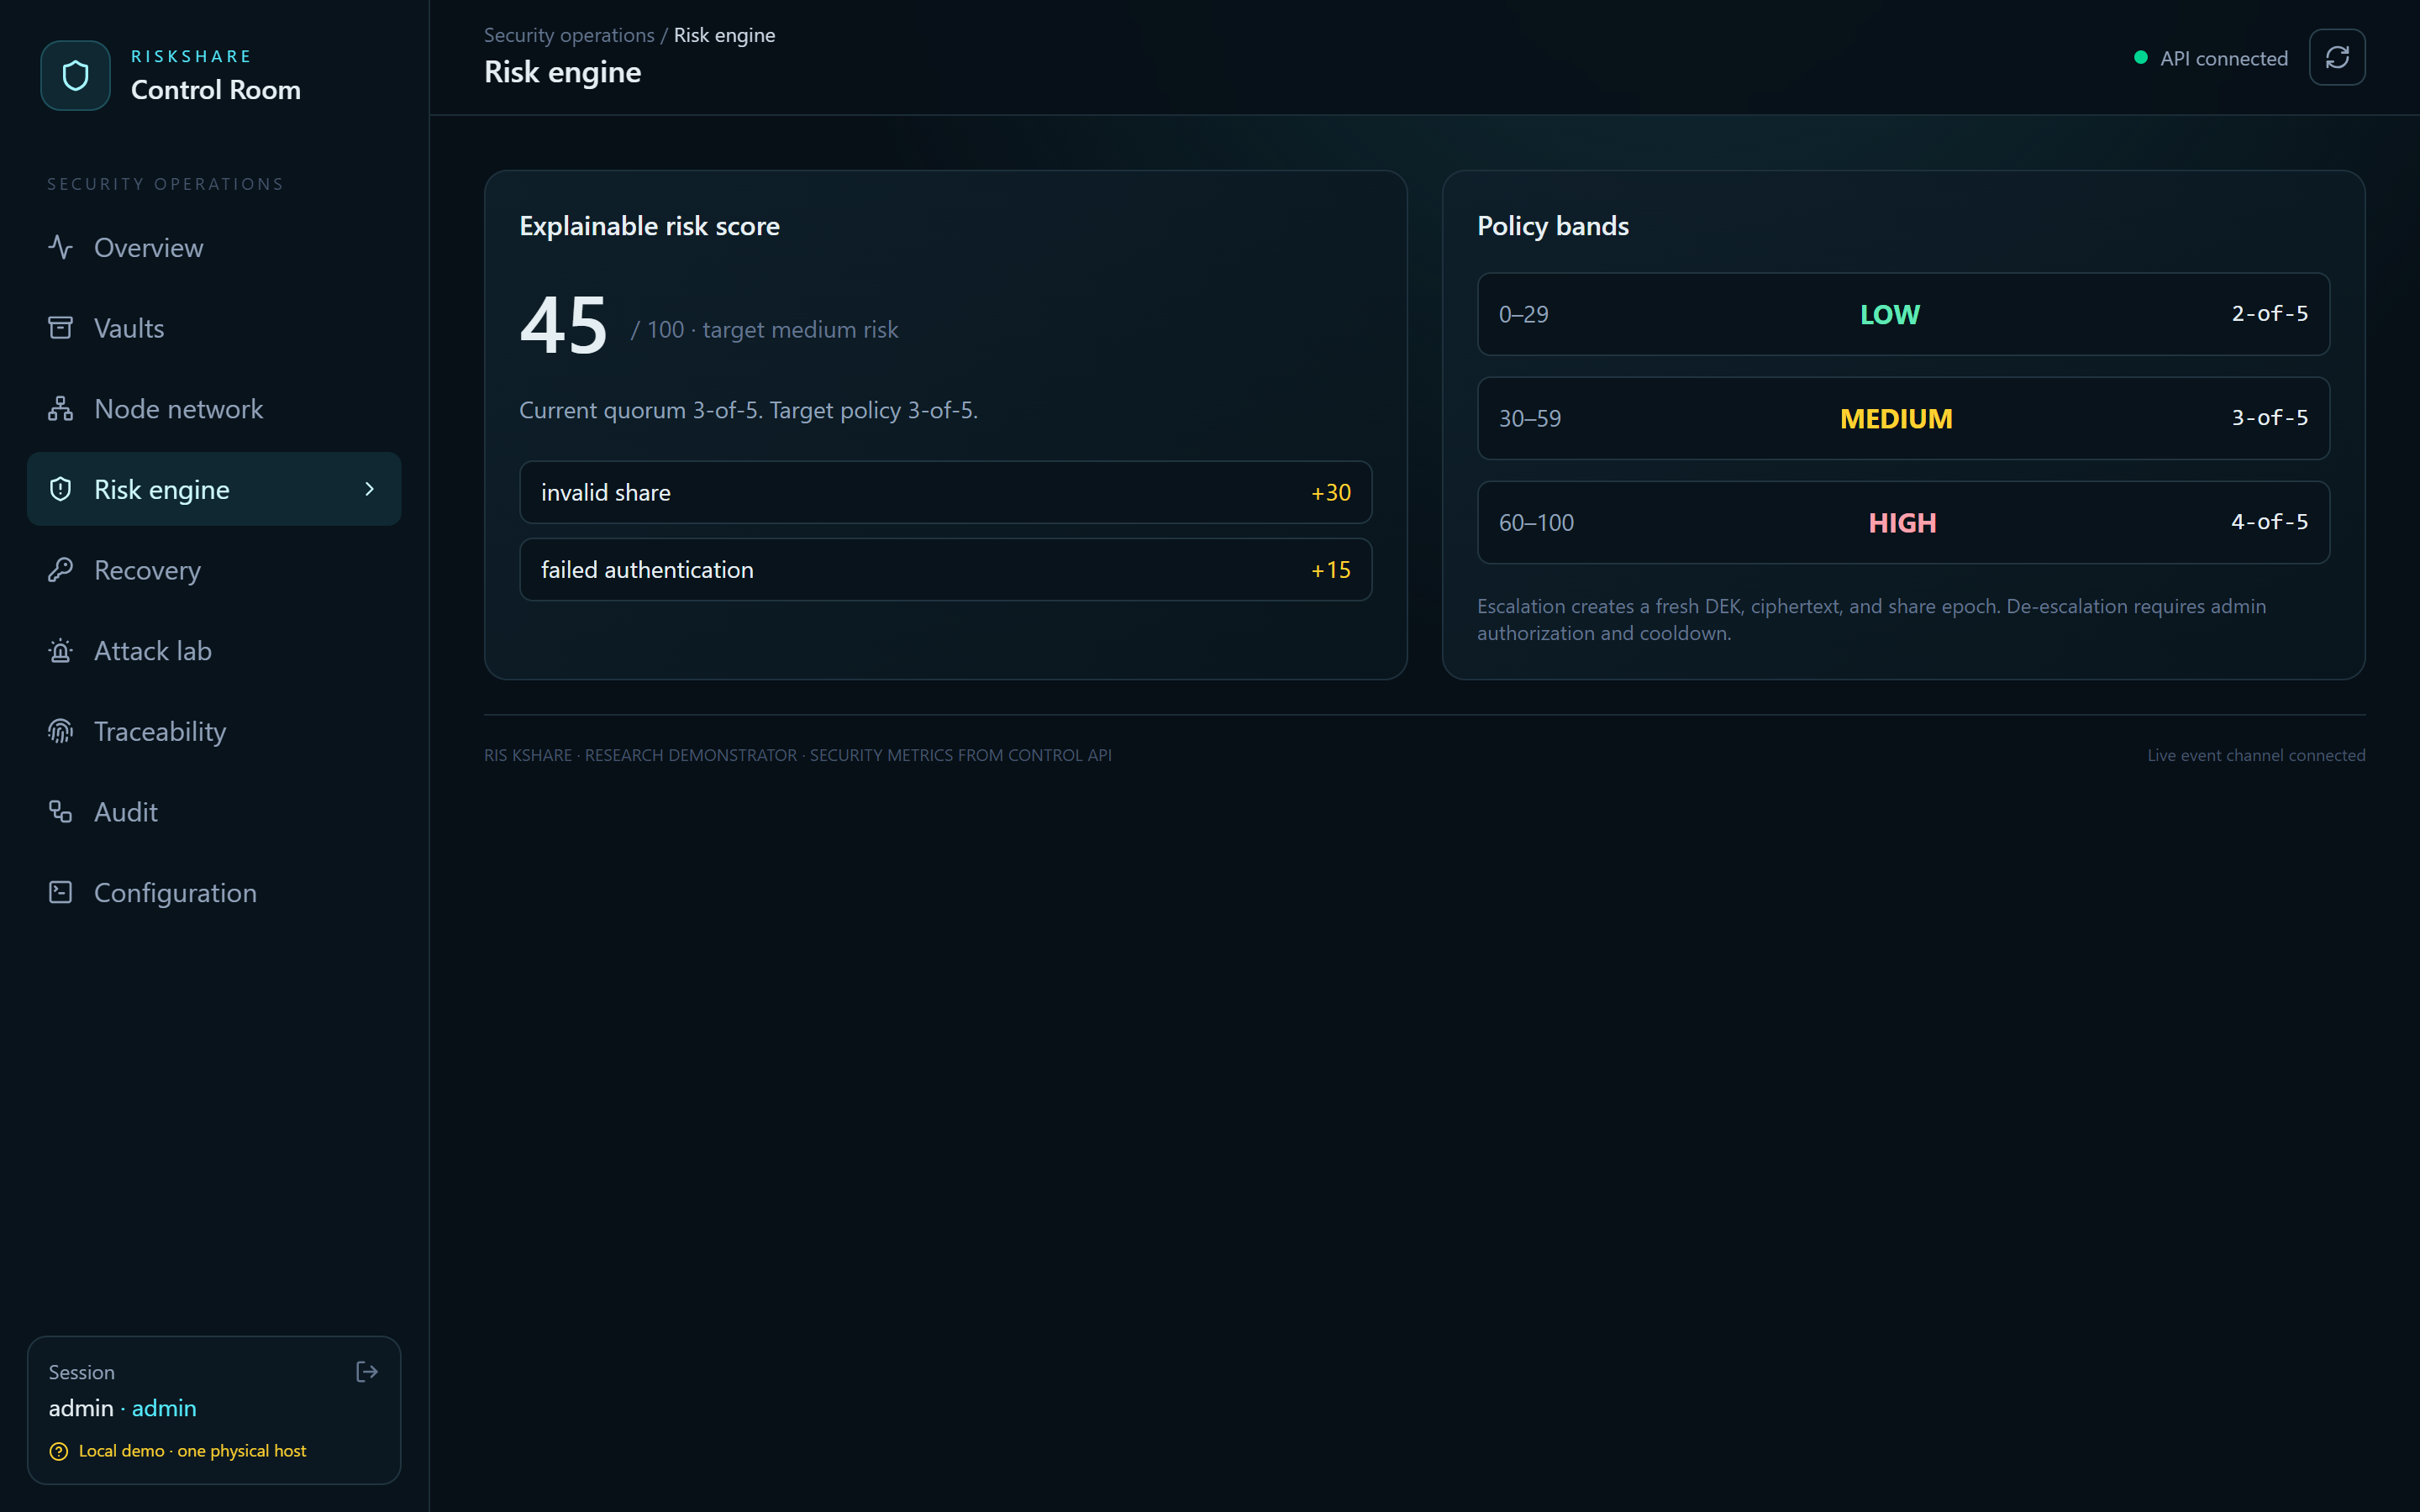
\includegraphics[width=0.485\textwidth]{figures/ui-risk.png}}\\[2mm]
\subfloat[Traceability: TTSS-II identifies node 1 and the proof passes public verification.]{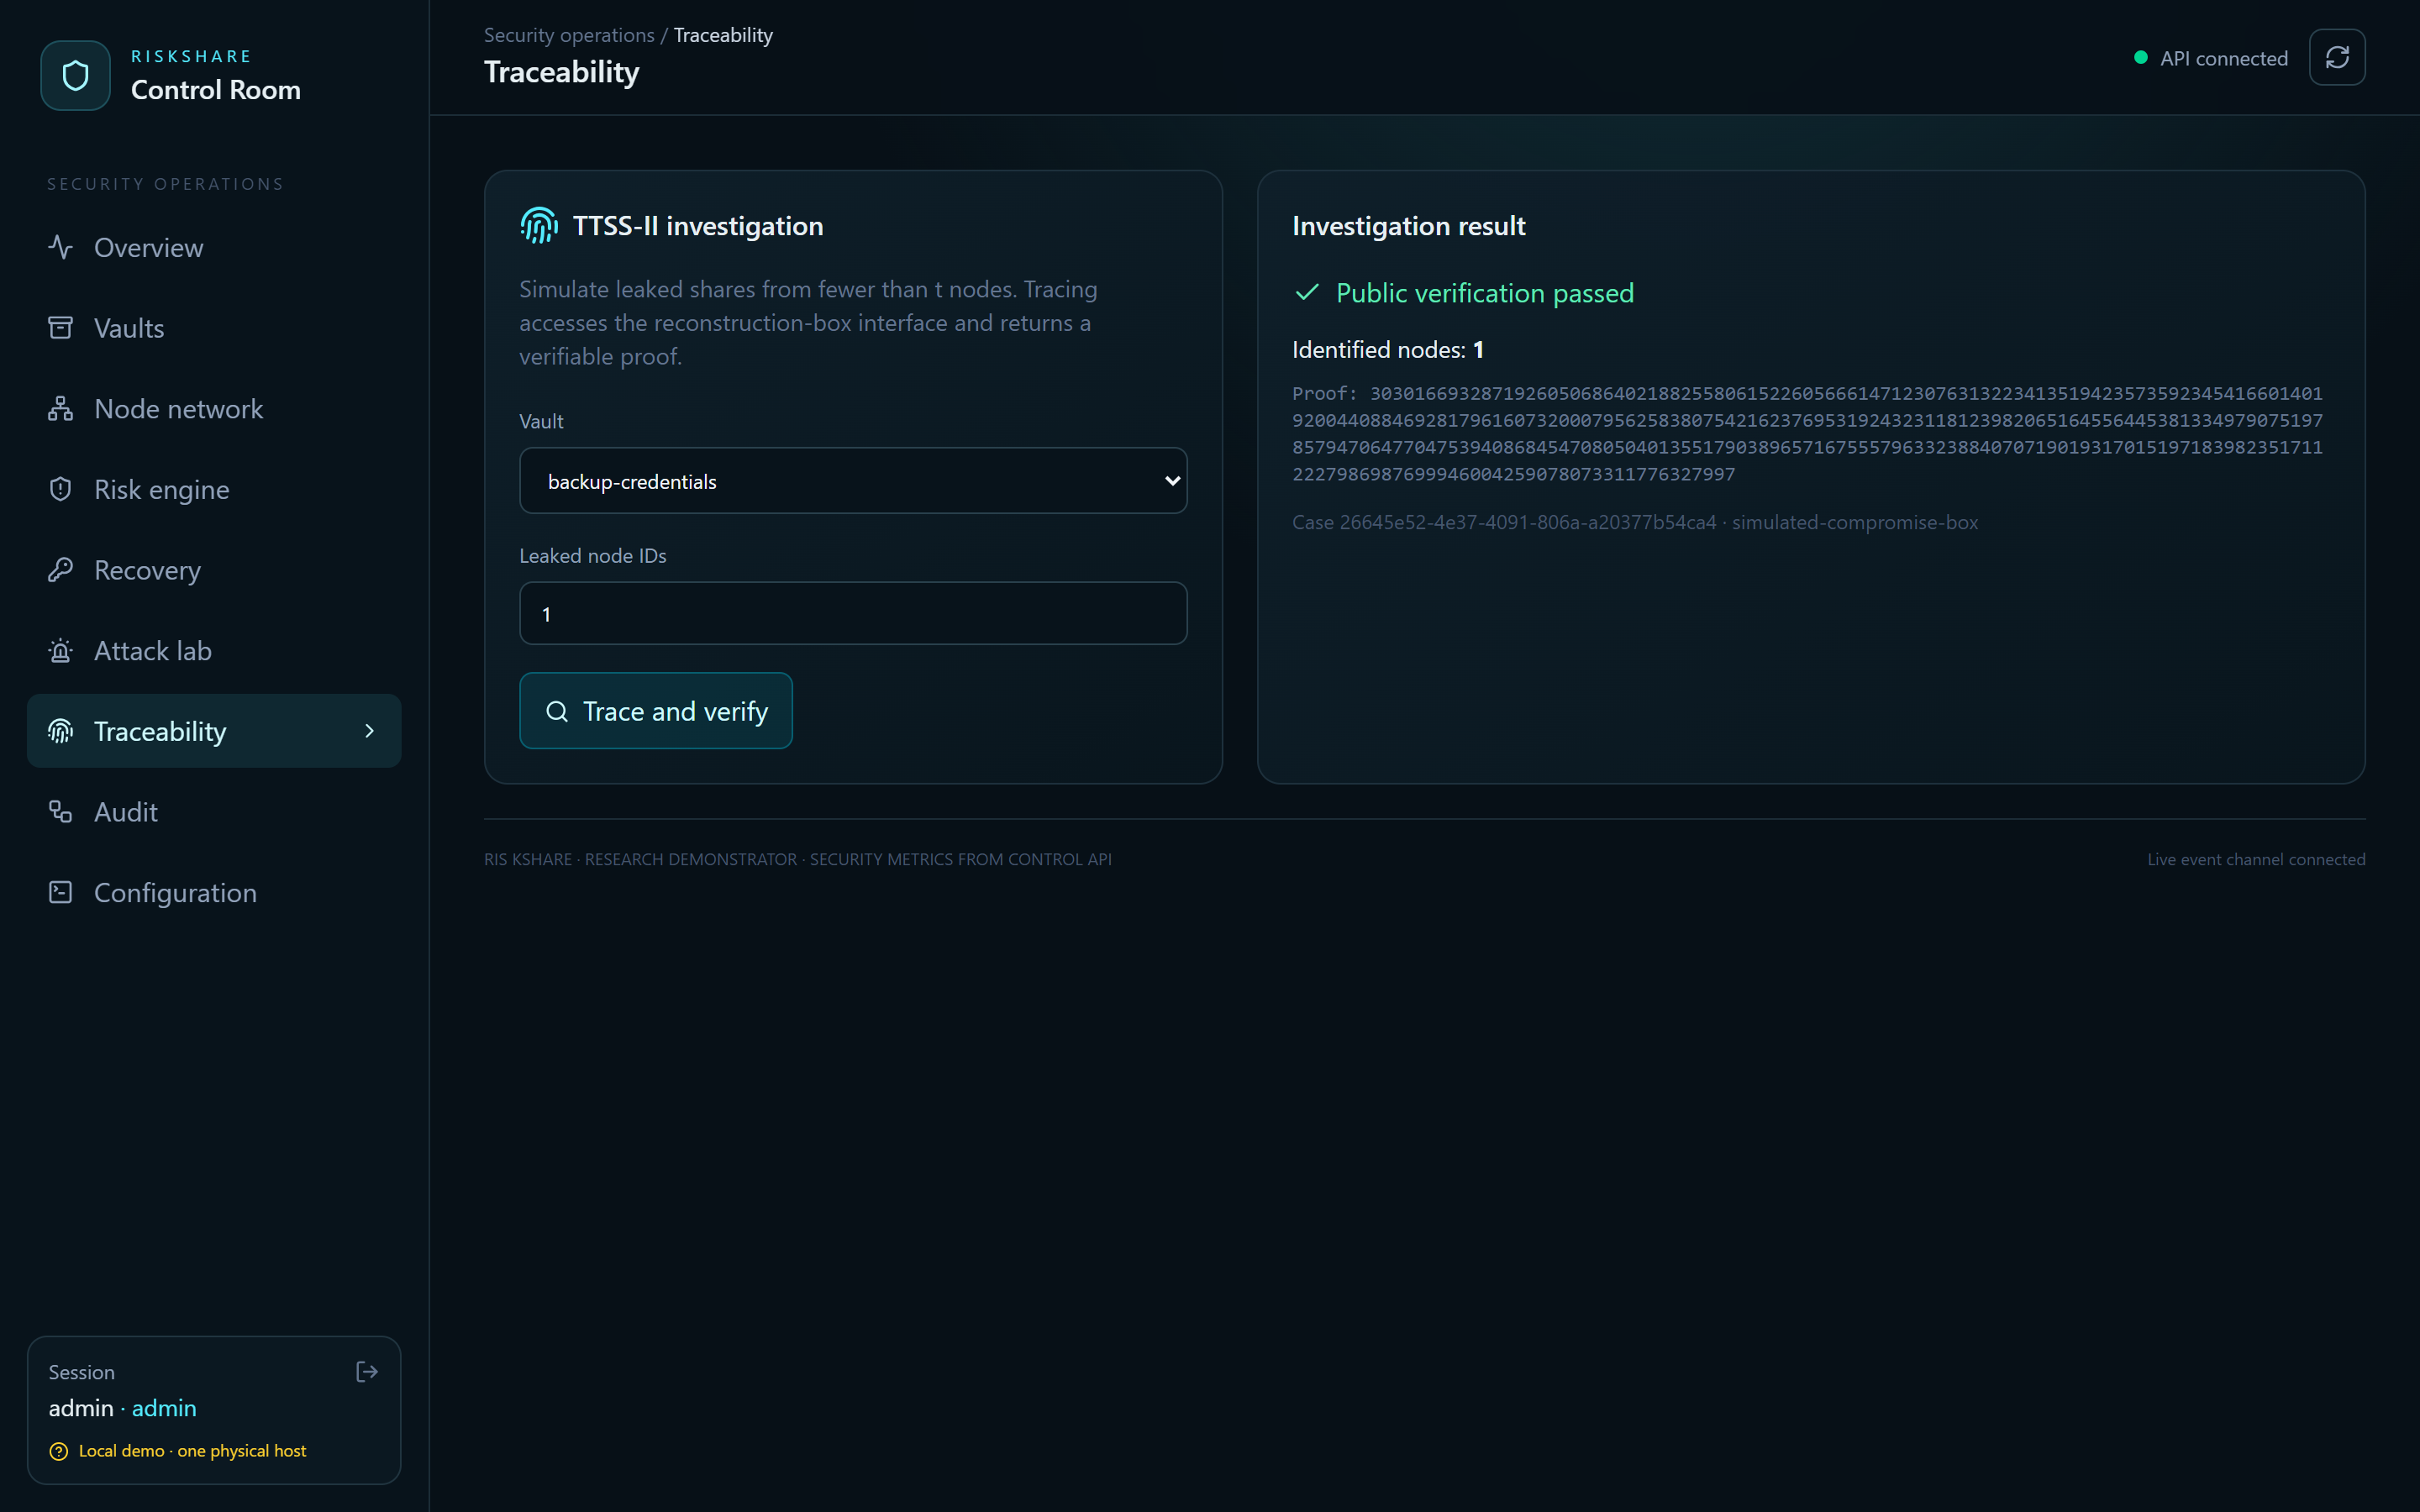
\includegraphics[width=0.485\textwidth]{figures/ui-trace.png}}\hfill
\subfloat[Audit: hash-chained events, including both epoch transitions; chain verified.]{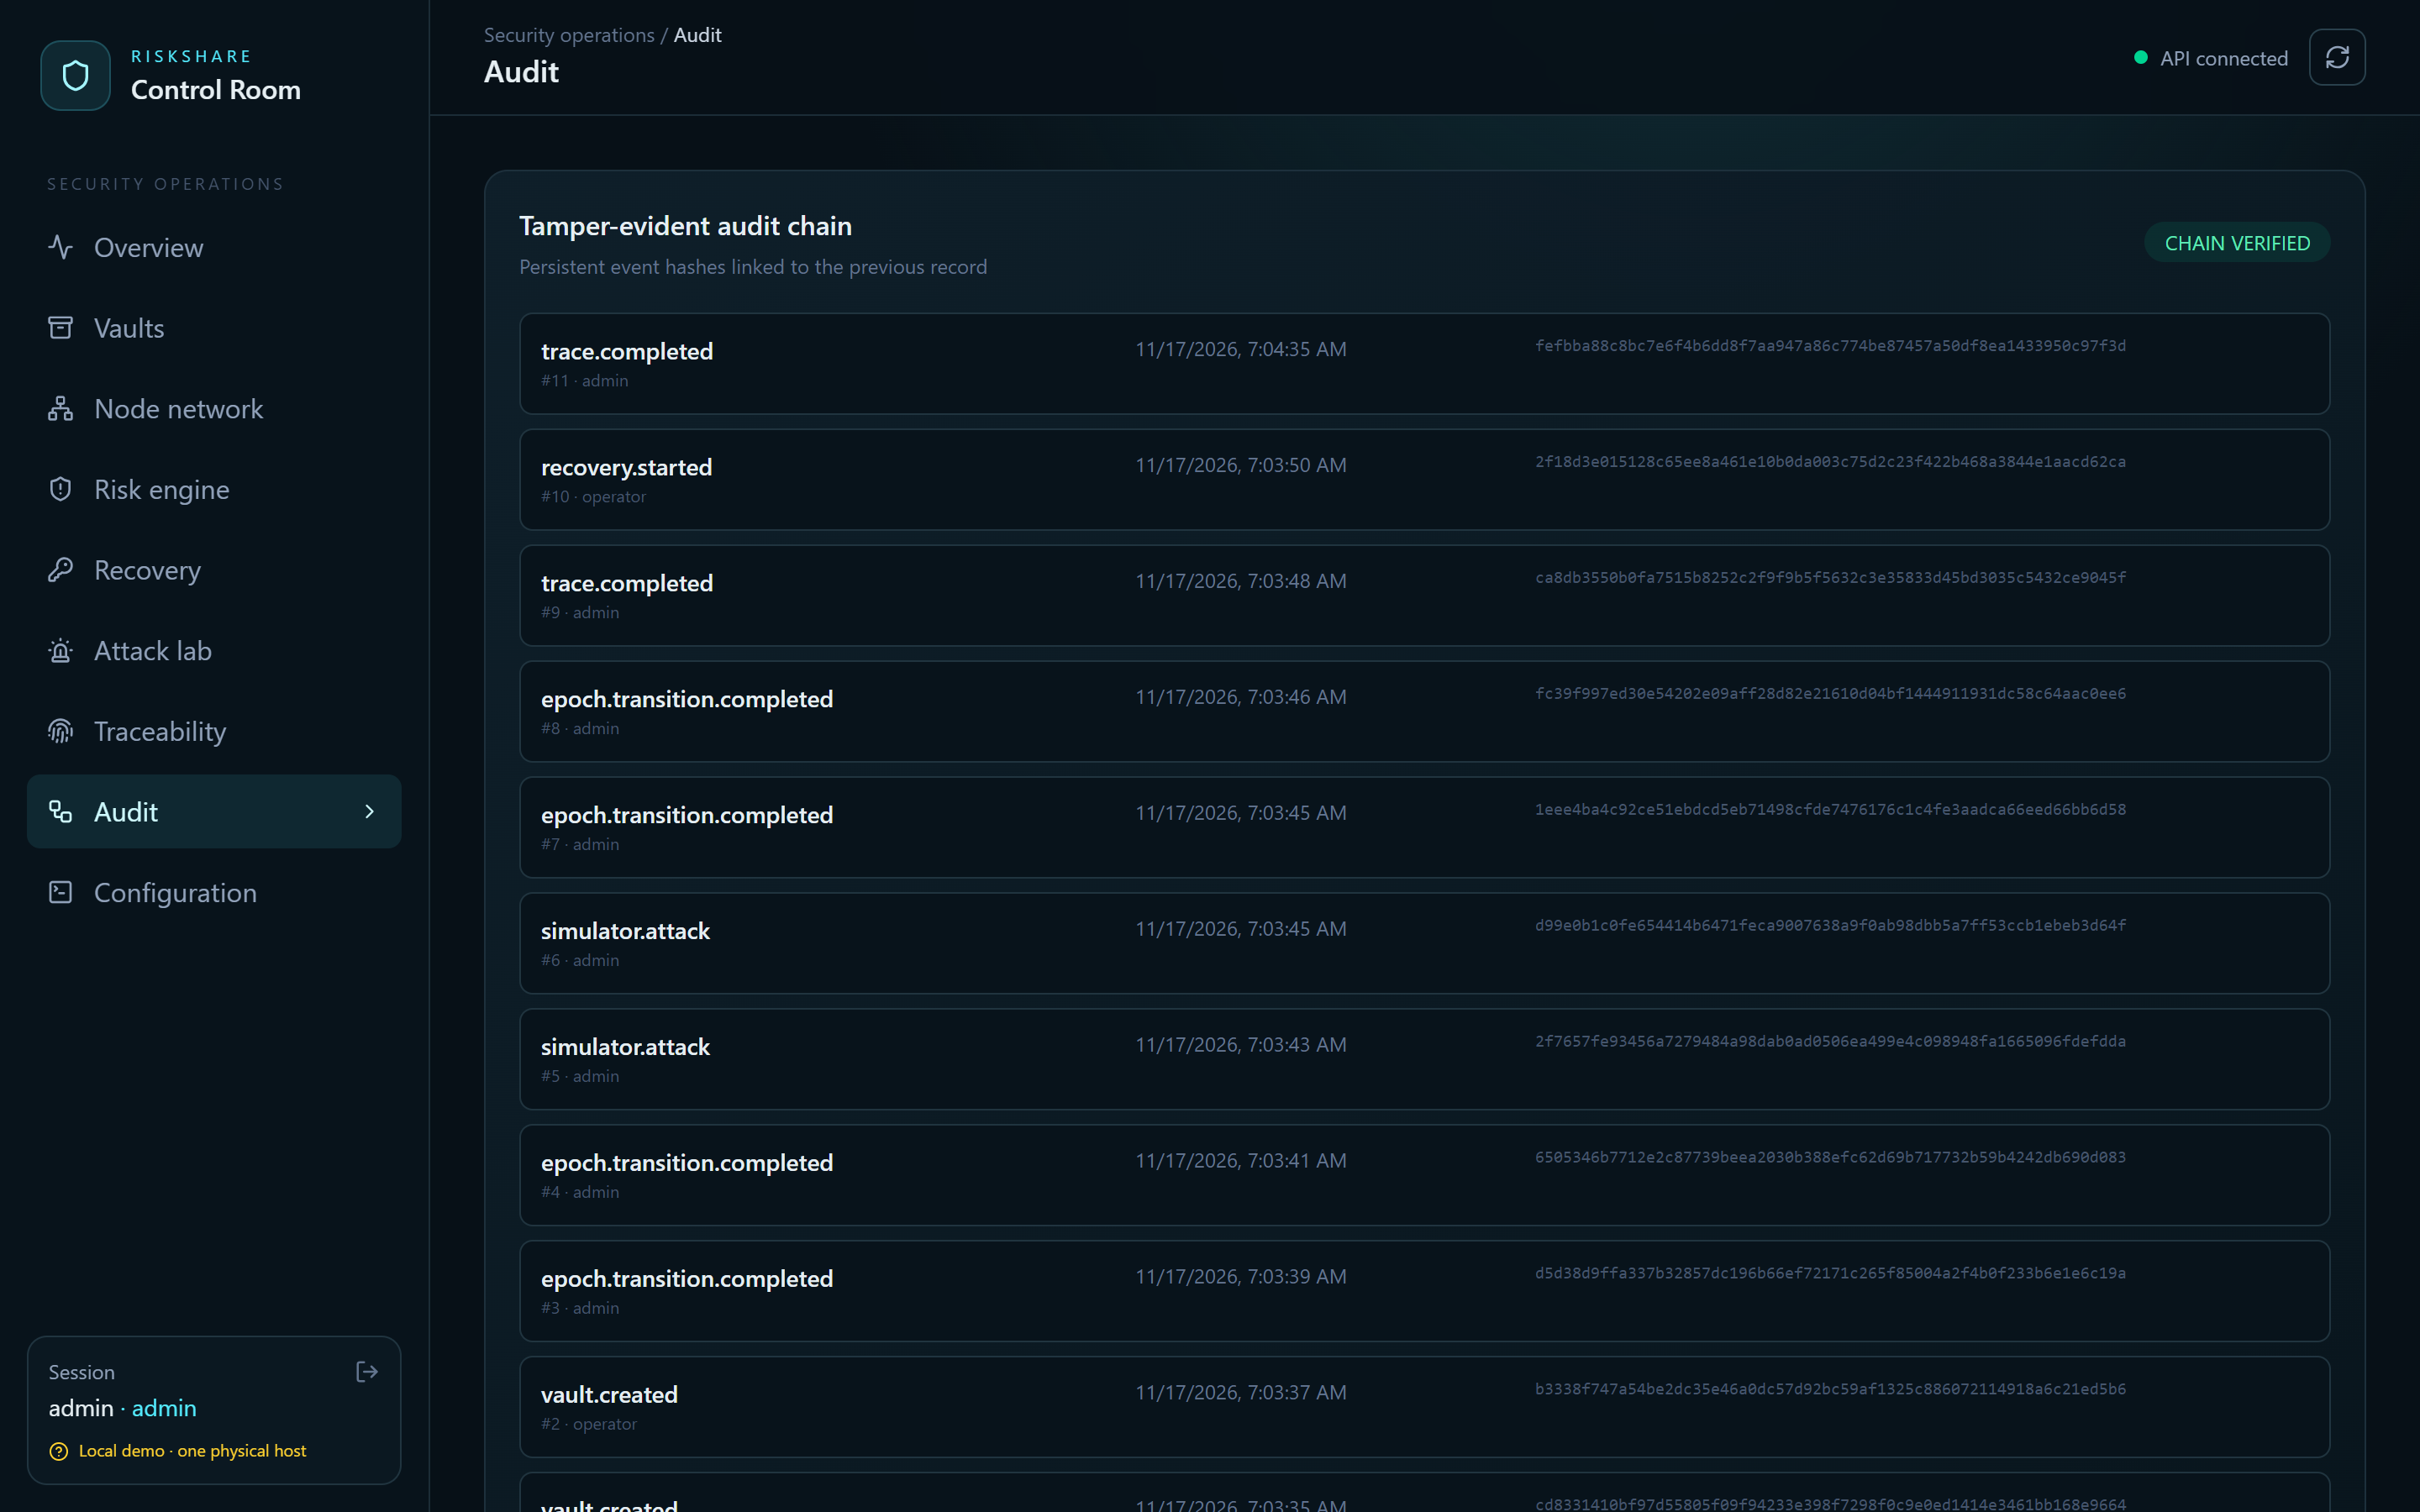
\includegraphics[width=0.485\textwidth]{figures/ui-audit.png}}
\caption{Screenshots of the \RS{} Control Room after the end-to-end demonstration (local research deployment, simulated events).}
\label{fig:ui}
\end{figure*}

% ===========================================================================
\section{Discussion and Limitations}
\label{sec:limits}

\paragraph*{Detector quality dominates} The adaptive gain in Fig.~\ref{fig:tradeoff} assumes that signals reflect the true number of compromised nodes~\eqref{eq:scen}. A stealthy adversary who triggers no events faces only the lenient threshold, so \RS{} complements a well-chosen baseline threshold and does not replace one. Conversely, false positives cost availability and rotations, which the cooldown limits but does not remove.

\paragraph*{Rotation is forward-looking} A fresh epoch protects data from the moment of activation. An adversary who reconstructed the DEK before escalation, or copied ciphertext and $t$ old shares, keeps that access. Rotation therefore narrows the window of exposure rather than undoing compromise, consistent with key-management practice~\cite{barker2020keymgmt}.

\paragraph*{Prototype scope} The local deployment runs five logical nodes on one host. The Compose deployment with separate containers and mTLS, and the Redis Streams integration, are implemented but were not executed end-to-end in our environment. Reconstruction still runs inside the API process rather than in an isolated worker. Rate limiting and token revocation are process-local, the tracing key is held in memory, and the audit chain has no external signed checkpoint. ABSS residues are not authenticated, so a malicious node can submit a wrong residue; this is detected only indirectly, through AES-GCM authentication failure. Verifiable sharing~\cite{feldman1987vss,pedersen1991vss} would close this gap.

\paragraph*{Evidence} The evaluation uses five trials and a deterministic scenario grid. Its rates are counts of scripted cases, not compromise probabilities, and the timings are single-machine measurements. Tests check behaviour; they do not prove secrecy, traceability or non-imputability, which rest on~\cite{leslie2025traceable} and need independent review of our instantiation.

\paragraph*{Future work} (i)~A top profile with $t=n$ or an explicit recovery freeze, to handle the $c=4$ column; (ii)~dealer-free threshold change~\cite{martin1999changing,steinfeld2007lattice} or proactive refresh~\cite{herzberg1995proactive}, to avoid central re-encryption; (iii)~per-node weights that exclude high-risk nodes from recovery quorums~\cite{nojoumian2010social}; (iv)~evaluation with realistic, noisy detectors and multi-host deployment.

% ===========================================================================
\section{Conclusion}
\label{sec:conclusion}
\RS{} shows that a secret-sharing threshold can respond to operational risk without unsound relabelling. Each change creates a fresh cryptographic epoch with a new key, new ciphertext and new shares under the new threshold, and is activated atomically or not at all. Built on the traceable Asmuth--Bloom schemes of Leslie and Dutta, the prototype integrates explainable risk scoring, fail-closed transitions, black-box leak tracing and tamper-evident audit. In our scripted evaluation the adaptive policy kept the attacker-reconstruction rate of the strictest fixed threshold while recovering more often, at a cost of tens of milliseconds per rotation. Whether this carries over to practice depends on detector quality, which is the next question to evaluate.

\section*{Artifact Availability}
The source code, test suite, experiment runner (\texttt{scripts/run\_experiments.py}), raw results (500 rows, CSV/JSON) and the scripts that regenerate every figure in this paper are included in the project repository.

\bibliographystyle{IEEEtran}
\bibliography{references}

\end{document}
